%%%%%%%%%%%%%%%%%%%%%%%%%%%%% Define Article %%%%%%%%%%%%%%%%%%%%%%%%%%%%%%%%%%
\documentclass{article}
%%%%%%%%%%%%%%%%%%%%%%%%%%%%%%%%%%%%%%%%%%%%%%%%%%%%%%%%%%%%%%%%%%%%%%%%%%%%%%%

%%%%%%%%%%%%%%%%%%%%%%%%%%%%% Using Packages %%%%%%%%%%%%%%%%%%%%%%%%%%%%%%%%%%
\usepackage{geometry}
\usepackage{graphicx}
\usepackage{amssymb}
\usepackage{amsmath}
\usepackage{amsthm}
\usepackage{empheq}
\usepackage{mdframed}
\usepackage{booktabs}
\usepackage{lipsum}
\usepackage{graphicx}
\usepackage{color}
\usepackage{psfrag}
\usepackage{pgfplots}
\usepackage{bm}
%%%%%%%%%%%%%%%%%%%%%%%%%%%%%%%%%%%%%%%%%%%%%%%%%%%%%%%%%%%%%%%%%%%%%%%%%%%%%%%

% Other Settings

%%%%%%%%%%%%%%%%%%%%%%%%%% Page Setting %%%%%%%%%%%%%%%%%%%%%%%%%%%%%%%%%%%%%%%
\geometry{a4paper}

%%%%%%%%%%%%%%%%%%%%%%%%%% Define some useful colors %%%%%%%%%%%%%%%%%%%%%%%%%%
\definecolor{ocre}{RGB}{243,102,25}
\definecolor{mygray}{RGB}{243,243,244}
\definecolor{deepGreen}{RGB}{26,111,0}
\definecolor{shallowGreen}{RGB}{235,255,255}
\definecolor{deepBlue}{RGB}{61,124,222}
\definecolor{shallowBlue}{RGB}{235,249,255}
%%%%%%%%%%%%%%%%%%%%%%%%%%%%%%%%%%%%%%%%%%%%%%%%%%%%%%%%%%%%%%%%%%%%%%%%%%%%%%%

%%%%%%%%%%%%%%%%%%%%%%%%%% Define an orangebox command %%%%%%%%%%%%%%%%%%%%%%%%
\newcommand\orangebox[1]{\fcolorbox{ocre}{mygray}{\hspace{1em}#1\hspace{1em}}}
%%%%%%%%%%%%%%%%%%%%%%%%%%%%%%%%%%%%%%%%%%%%%%%%%%%%%%%%%%%%%%%%%%%%%%%%%%%%%%%

%%%%%%%%%%%%%%%%%%%%%%%%%%%% English Environments %%%%%%%%%%%%%%%%%%%%%%%%%%%%%
\newtheoremstyle{mytheoremstyle}{3pt}{3pt}{\normalfont}{0cm}{\rmfamily\bfseries}{}{1em}{{\color{black}\thmname{#1}~\thmnumber{#2}}\thmnote{\,--\,#3}}
\newtheoremstyle{myproblemstyle}{3pt}{3pt}{\normalfont}{0cm}{\rmfamily\bfseries}{}{1em}{{\color{black}\thmname{#1}~\thmnumber{#2}}\thmnote{\,--\,#3}}
\theoremstyle{mytheoremstyle}
\newmdtheoremenv[linewidth=1pt,backgroundcolor=shallowGreen,linecolor=deepGreen,leftmargin=0pt,innerleftmargin=20pt,innerrightmargin=20pt,]{theorem}{Theorem}[section]
\theoremstyle{mytheoremstyle}
\newmdtheoremenv[linewidth=1pt,backgroundcolor=shallowBlue,linecolor=deepBlue,leftmargin=0pt,innerleftmargin=20pt,innerrightmargin=20pt,]{definition}{Definition}[section]
\theoremstyle{myproblemstyle}
\newmdtheoremenv[linecolor=black,leftmargin=0pt,innerleftmargin=10pt,innerrightmargin=10pt,]{problem}{Problem}[section]
%%%%%%%%%%%%%%%%%%%%%%%%%%%%%%%%%%%%%%%%%%%%%%%%%%%%%%%%%%%%%%%%%%%%%%%%%%%%%%%

%%%%%%%%%%%%%%%%%%%%%%%%%%%%%%% Plotting Settings %%%%%%%%%%%%%%%%%%%%%%%%%%%%%
\usepgfplotslibrary{colorbrewer}
\pgfplotsset{width=8cm,compat=1.9}
%%%%%%%%%%%%%%%%%%%%%%%%%%%%%%%%%%%%%%%%%%%%%%%%%%%%%%%%%%%%%%%%%%%%%%%%%%%%%%%

%%%%%%%%%%%%%%%%%%%%%%%%%%%%%%% Title & Author %%%%%%%%%%%%%%%%%%%%%%%%%%%%%%%%
\title{Ejercicio 28}
\author{Rodrigo Miranda}
%%%%%%%%%%%%%%%%%%%%%%%%%%%%%%%%%%%%%%%%%%%%%%%%%%%%%%%%%%%%%%%%%%%%%%%%%%%%%%%

\begin{document}
    \maketitle Ejercicio 28 - Guia de ejercicios 1
    \begin{figure}[ht]
        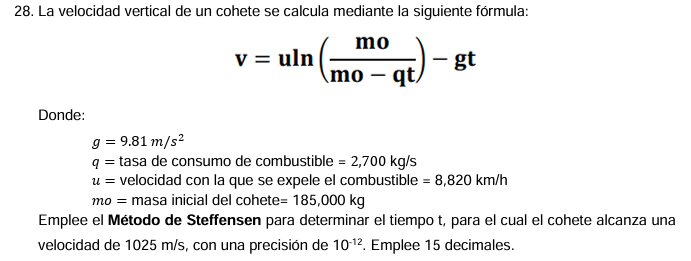
\includegraphics[scale=0.9]{img/stf28_1.png}
    \end{figure}
    \\Debemos antes que nada convertir el valor de u. $u=8820 km/h = 2.45km/s= 2450m/s$
    
    Iniciemos encontrando un intervalo, para ello debemos hacer f(x)=0.
    \\$ f(x)=uln(\frac{mo}{mo-qt})-gt-v=0$
    \\Una vez despejado, vamos a graficar en matlab. Pero antes, debemos declarar las variables con los datos que el ejercicio nos brinda.
    Tal que:
    $
    g=9.81;\\
    q=2700;\\
    u=2450;\\
    mo=185000;\\
    v=1025;\\
    f=u*log(mo/(mo-q*x))-g*x-v;
    $
    
    \begin{figure}[ht]
        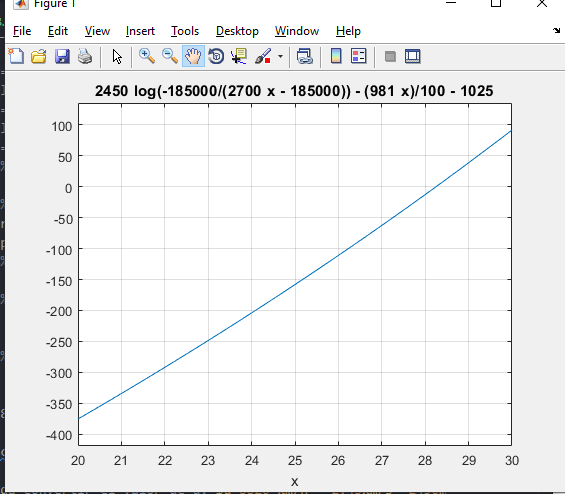
\includegraphics[scale=0.5]{img/stf28_2.png}{\\Graficando podemos ir observando que el intervalo donde se encuentra la raiz es [28,29]}
    \end{figure}
    \pagebreak
    \noindent Procedemos a encontrar nuestra ecuacion g(x)=x para evaluarla y graficarla en el intervalo encontrado.
Para esto, iniciaremos sumando x cada lado de la ecuacion, tal que:
$g(x)=uln(\frac{mo}{mo-qt})-gt-v+x$

Validemos graficando en matlab: $gx=u*log(mo/(mo-q*x))-g*x-v+x$
\begin{figure}[ht]
    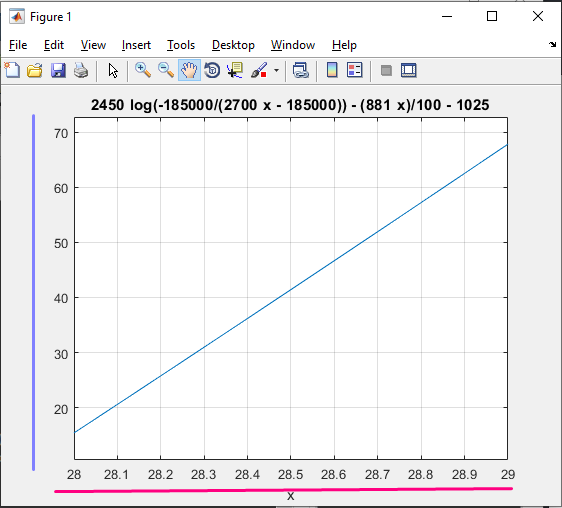
\includegraphics[scale=0.5]{img/stf28_3.png}
    
\end{figure}
\\Debemos observar detenidamente el grafico, para cumplir el metodo los valores en x Y y
    deben ser iguales, sin embargo, vemos que para un x=28,y=20; por lo tanto se separan y por
    mucho
\\Intentaremos ahora despejar x, del factor gx $(gt)$. De manera que:

$x=\frac{uln(\frac{mo}{mo-qt})-v}{g}$
\\Igresado en matlab: $gx=(u*log(mo/(mo-q*x))-v)/g$. Grafiquemos para comprobar el metodo:
\begin{figure}[ht]
    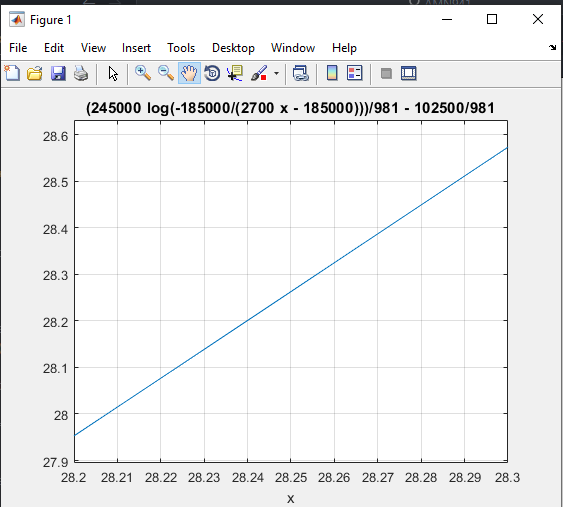
\includegraphics[scale=0.7]{img/stf28_6.png}{\\El metodo se cumple, podemos proceder a ejecutar el programa en matlab para encontrar la raiz.}
    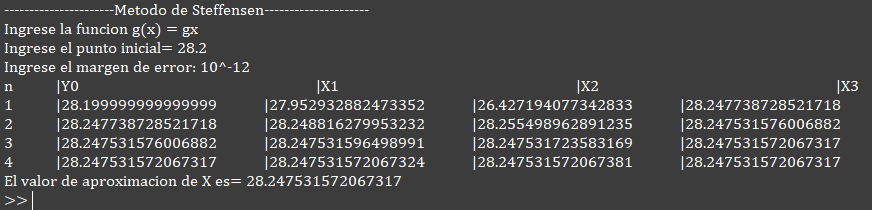
\includegraphics[scale=0.6]{img/stf28_7.png}{\\El tiempo que al cohete le toma alcanzar $1025m/s$ es t=28.247531572067317}
\end{figure}

\end{document}